\documentclass{standalone}
%% Load packages
\usepackage{tikz}
\usetikzlibrary{calc}
\usetikzlibrary{trees}

\begin{document}
	\bf\large
	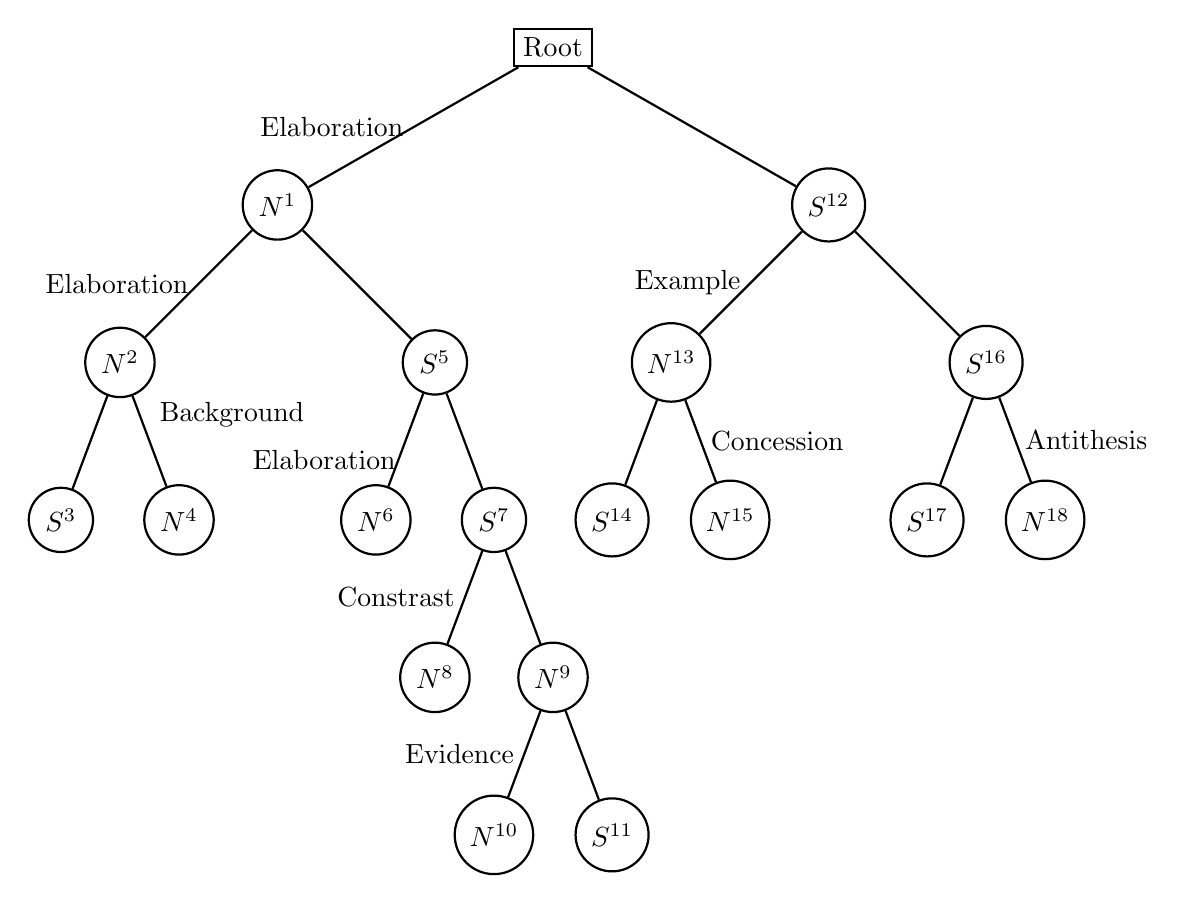
\begin{tikzpicture}[level distance=2cm,
	level 1/.style={sibling distance=7cm},
	level 2/.style={sibling distance=4cm},
	level 3/.style={sibling distance=1.5cm},
	root node/.style={thick, draw},
	tree node/.style={thick, circle,draw},
	every child node/.style={tree node}]
	
	\node[root node] (Root) {Root}
	child[thick] {
		node[tree node] {$N^1$} 
		child { node[tree node] {$N^2$} 
			child { node[tree node] {$S^3$} }
			child { node[tree node] {$N^4$} edge from parent node[right] {\raisebox{1.75pc}{Background}} }
			edge from parent node[left] {Elaboration}
		}
		child { node[tree node] {$S^5$} 
			child { node[tree node] {$N^6$} edge from parent node[left] {\raisebox{-1.75pc}{Elaboration}} } 
			child { node[tree node] {$S^7$} 
				child { node[tree node] {$N^8$} edge from parent node[left] {Constrast} }
				child { node[tree node] {$N^9$} 
					child { node[tree node] {$N^{10}$} edge from parent node[left] {Evidence} }
					child { node[tree node] {$S^{11}$} }
				}
			}
		}
		edge from parent node[left] {Elaboration}
	}
	child[thick] {
		node[tree node] {$S^{12}$}
		child { node[tree node] {$N^{13}$} 
			child { node[tree node] {$S^{14}$} }
			child { node[tree node] {$N^{15}$} edge from parent node[right] {Concession} }
			edge from parent node[left] {Example}
		}
		child { node[tree node] {$S^{16}$}
			child { node[tree node] {$S^{17}$} }
			child { node[tree node] {$N^{18}$} edge from parent node[right] {Antithesis}}	
		}
	};
	\end{tikzpicture}
\end{document}